\documentclass{scrartcl}
\usepackage{float}
\usepackage[utf8]{inputenc}
\usepackage[T1]{fontenc}
\usepackage{lmodern}
\usepackage[ngerman]{babel}
\usepackage{amsmath}
\usepackage{mathtools}
\usepackage{amssymb}
\usepackage{stmaryrd}
\usepackage{blindtext}
\title{7. AuD Uebung}
\author{Adrian Hille}
\begin{document}
\Large 7. AuD \"Ubung (25. November 2015)\\
\\
\normalsize
Aufgabe 4b)\\
$\binom{\varnothing}{\varnothing} \xmapsto{\text{f}}
 \binom{\{\varepsilon \}}{\varnothing} \xmapsto{\text{f}}
 \binom{\{\varepsilon \}}{\{ c\}} \xmapsto{\text{f}}
 \binom{\{ \varepsilon , acb\}}{\{c\}} \xmapsto{\text{f}}
 \binom{\{ \epsilon, acb\}}{\{acbc,c,cacb\}} \xmapsto{\text{f}}
 \binom{\{ aacbcb,acb,acacbb, \epsilon\}}{\{acbc,c,cacb\}}$\\

W($\varepsilon$): a a a b b b \\
\\
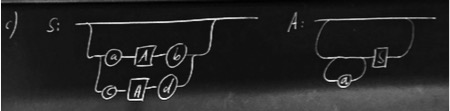
\includegraphics{syntax01.jpg}
\\

\begin{tabular}[c]{c|c}
	Objekt & G\"ultigkitsbereich\\
	\hline
	g & 5 -39\\
	\hline
	f & 16-39\\
	\hline
	i in f & 18-27\\
	\hline
	a (global) & 3-39\\
	\hline
	n,c in main & 31-39\\
	\hline
	j,k in g & 5-14\\
	\hline
	m,d in f & 16-27\\
\end{tabular}
\\
\\
\begin{tabular}[c]{c|r|c|c|c|c|c|c|c|c|c|c}
	Haltepunkt & RM & 1 & 2 & 3 & 4 & 5 & 6 & 7 & 8 & 9 & 10\\
	\hline
	label 6 & - & a=6 & n=6 & c=0 &  & d=3 & i=2 &  &  &  & \\
	\hline
	label 4 & 2;3 &  &  &  & m=6 & d=3 & i=2 &  &  &  & \\
	\hline
	label 1 & 2;3 &  &  &  &  &  &  & j $\#$6  & k=6 &  & \\
	\hline
	label 3 & 2;3 &  &  &  &  &  &  & j $\#$6  & k=6 &  & \\
	\hline
	label 5 & 3 &  &  & 1 & m=3 & d $\#$3 & i=2 &  &  &  & \\
	\hline
	label 1 & 2;3 &  &  &  &  &  &  & j $\#$6  & k=3 &  & \\
	\hline
	label 1 & 1;2;3 &  &  &  &  &  & 3 &  &  & j $\#$6 & k=3 \\
	\hline
	label 3 & 1;2;3 &  &  &  &  &  &  &  &  & j $\#$6 & k=3 \\
	\hline
	label 2 & 2;3 &  &  &  &  &  &  &j $\#$6  & k=3 &  &  \\
	\hline
	label 5 & 3 &  &  &  & m=1 & d$\#$3 & i=2 &  &  &  & \\
	\hline
	label 7 & - & a=6 & n=6 & c=2 &  &  &  &  &  &  & \\
\end{tabular}
\end{document}